\section{熔解和凝固}\label{sec:4-1}

\begin{wrapfigure}{r}{5cm}
    \centering
    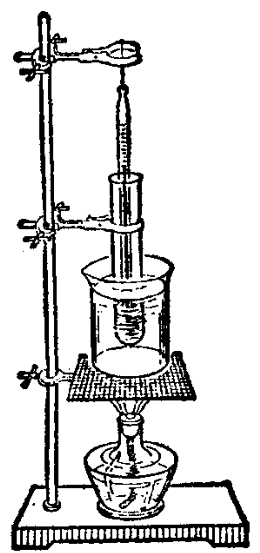
\includegraphics[width=4cm]{../pic/czwl2-ch4-1}
    \caption{观察萘的熔解}\label{fig:4-1}
\end{wrapfigure}

这一节我们来研究物质从固态变成液态或者由液态变成固态的规律。
物质从固态变成液态,叫做\textbf{熔解};
    从液态变成固态,叫做\textbf{凝固}。
现在用实验来研究熔解和凝固的过程。

\xiaobiaoti{熔点和凝固点}
把装有萘的试管放在盛有水的烧杯里,在试管中插入温度计,用酒精灯通过烧杯和水均匀地给萘加热(图 \ref{fig:4-1})。
萘吸收热量,温度不断升高,当温度上升到 80 ℃ 时,开始熔解。
在熔解过程中,虽然继续加热,但萘的温度却保持 80 ℃ 不变,直到完全熔解后,温度才继续上升。
这表明,萘是在一定的温度下熔解的。

把松香装在试管里,做同样的实验,可以看出,固态的松香先是变软,然后逐渐变成液态。
松香在整个熔解过程中,温度不断上升,并不保持一定的温度。
可见,松香没有一定的熔解温度。

固体分晶体和非晶体两类。
萘、冰、石英、水晶、食盐、海波、各种金属、大多数矿石都是晶体。
松香、玻璃、蜂蜡、沥青等都是非晶体。

实验表明,
所有的晶体都跟萘一样,在一定的温度下熔解;
所有的非晶体都跟松香一样,没有一定的熔解温度。

晶体熔解时的温度叫做\textbf{熔点}。晶体不同,熔点也不同。

\begin{table}[H]
    \centering
    \caption*{几种物质的熔点(℃)}
    \begin{tblr}{
        colspec={|ll|ll|ll|},
        columns={colsep+=0.5em},
        column{6}={mode=math},
    }
        \hline
        钨 & 3410 & 铝 & 660 & 固态水银 & -39 \\
        纯铁 & 1535 & 铅 & 327 & 固态酒精 & -117 \\
        钢 & 1130~1400 & 锡 & 232 & 固态氮 & -210 \\
        铸铁 & 约 1200 & 萘 & 80 & 固态氢 & -259 \\
        铜 & 1083 & 海波 & 48 & 固态氨 & -272 \\
        金 & 1064 & 冰 & 0 &  &  \\
        \hline
    \end{tblr}
\end{table}


在图 \ref{fig:4-1} 所示的实验中,在萘熔解成液体以后,如果停止对烧杯加热,液态萘的温度就不断降低。
当温度降到 80 ℃ 时,萘开始凝固。萘在凝固过程中,温度保持不变,直到全部凝固后,温度才又开始下降。
可见,晶体不但在一定的温度下熔解,也在一定的温度下凝固。
晶体凝固时的温度叫做\textbf{凝固点}。同一物质的凝固点跟它的熔点相同。


\begin{figure}[htbp]
    \centering
    %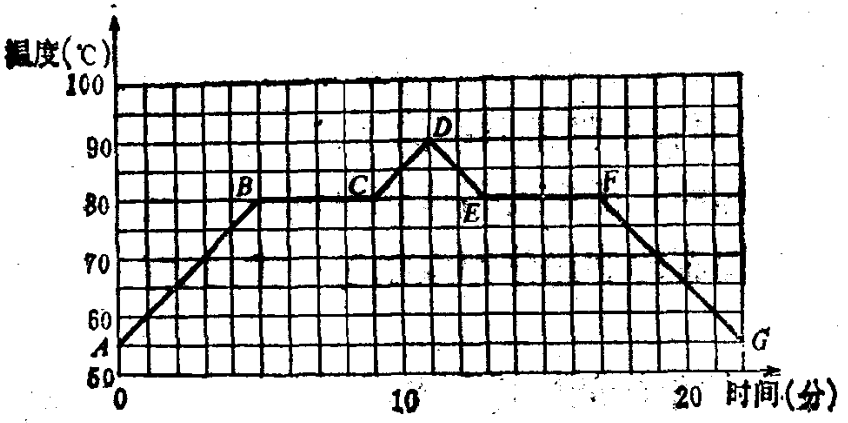
\includegraphics[width=0.6\textwidth]{../pic/czwl2-ch4-2.old}
    \begin{tikzpicture}[>=Stealth, scale=0.8]
    \draw [thick,->] (0, 0) -- (12, 0) node[anchor=north] {时间(分)};
    \draw [thick,->] (0, 0) -- (0, 6) node[anchor=east] {温度(℃)};

    \foreach \x in {0.5, 1, 1.5, ..., 11} {
        \draw (\x, 0) -- (\x, 5);
    }

    \foreach \y in {0.5, 1, 1.5, ..., 5} {
        \draw (0, \y) -- (11, \y);
    }

    \foreach \x in {0,10,20} {
        \draw (\x/2,0.2) -- (\x/2,0) node[anchor=north] {$\x$};
    }
    \foreach \y in {50,60,...,100} {
        \tikzmath{
            \v = (\y-50)/10;
        }
        \draw (0.2,\v) -- (0,\v) node[anchor=east] {$\y$};
    }

    \coordinate (A) at (0, 0.5);
    \coordinate (B) at (2.5, 3);
    \coordinate (C) at (4.5, 3);
    \coordinate (D) at (5.5, 4);
    \coordinate (E) at (6.5, 3);
    \coordinate (F) at (8.5, 3);
    \coordinate (G) at (11, 0.5);

    \draw [very thick] (A) -- (B) -- (C) -- (D) -- (E) -- (F) -- (G);
    \foreach \n/\x/\y in {
            A/-0.3/0, B/-0.3/0.3, C/-0.3/0.3, D/0.3/0.3,
            E/-0.3/-0.3, F/0.3/0.3, G/0.3/0} {
        \coordinate (P) at (\x, \y);
        \node [fill=white, inner sep=0pt, font=\footnotesize] at ($(P) + (\n)$) {$\n$};
        \draw [fill=black] (\n) circle (2pt);
    }
\end{tikzpicture}

    \caption{萘的熔解和凝固图象}\label{fig:4-2}
\end{figure}

\xiaobiaoti{熔解和凝固图象}
物质的熔解和凝固过程,可以用图象来表示。图 \ref{fig:4-2}\footnotemark 是萘的熔解和凝固图象。
\footnotetext{注:原书的图模糊不清,我使用 tikz 绘制了一个图片。} % 原书图片 保存为 pic 目录下的 czwl2-ch4-2.old.png
图中,横坐标表示时间,纵坐标表示温度,从萘的温度是 55 ℃ 开始计时,
图象 $ABCDEFG$ 表示了萘在加热和冷却程中,它的温度随时间而变化的情况。
其中,$BC$ 部分表示萘的熔解过程,$EF$ 部分表示疑固过程。
从图中可以看出,萘在熔解和凝固过程中温度保持不变,它的熔点和凝固点都是 80 ℃。
象这样用图象来表示物理量的变化情况,是物理学中常用的方法。
在物理实验中,就常常用图象把实验结果表示出来,它能直观地表示出物理量的变化规律。


\xiaobiaoti{熔解热}
晶体在熔解过程中虽然温度保持不变,但要继续给它加热,熔解过程才能完成。
这表明晶体在熔解过程中要吸收热量。
单位质量的某种晶体,在熔点变成同温度的液体时吸收的热量,叫做这种物质的\textbf{熔解热}。
液体在凝固时要放出热量。
单位质量的液体,在凝固点变成同温度的晶体时放出的热量,等于它的熔解热。
例如,冰的熔解热是 80 卡/克, 1 克水在 0 ℃ 疑固成 0 ℃ 的冰放出的热量也是 80 卡。



\lianxi

(1) 在很冷的地区,为什么不用水银温度计而用酒精温度计来测量气温?

(2) 要使热的物体冷却,用质量相等的 0 ℃ 的水或 0 ℃ 的冰,哪一种效果好些?为什么?

(3) 把正在熔解的冰拿到 0 ℃ 的房间里,冰能不能继续熔解?为什么?
把装在瓶里的水放在 0 ℃ 的房间里,水能不能结冰?为什么?

(4) 电灯泡发光时灯丝的温度达到 2000 ℃。能用铁、金、铅来制造电灯泡的灯丝吗?
如果由你来挑选,你准备选哪种金属来制造电灯泡的灯丝?说明你的理由。


